
\begin{itemize}
\item Consider an experiment in which each student in a class of 60 rolls a die 100 times.
\item Each score is recorded, and a total score is calculated.
\item As the expected value of rolled die is 3.5, the expected total is 350 for each student.
\item At the end of the experiment the students reported their totals.
\item The totals were put into ascending order, and tabulated as follows (next slide).
\end{itemize}

\begin{center}
\begin{tabular}{|c c c c c c c c c c|}
\hline
% after \\: \hline or \cline{col1-col2} \cline{col3-col4} ...
307 & 321 & 324 & 328 & 329 & 330 & 334 & 335 & 336 &337 \\
337 & 337 & 338 & 339 & 339 & 342 & 343 & 343 & 344 &344 \\
346 & 346 & 347 & 348 & 348 & 348 & 350 & 351 & 352 &352 \\
353 & 353 & 353 & 354 & 354 & 356 & 356 & 357 & 357 &358 \\
358 & 360 & 360 & 361 & 362 & 363 & 365 & 365 & 369 &369 \\
370 & 370 & 374 & 378 & 381 & 384 & 385 & 386 & 392 &398 \\
\hline
\end{tabular}
\end{center}
\normalsize
\begin{itemize}
\item What proportion of outcomes are less than or equal to 330? \\ (Answer: $10\%$)
\item What proportion of outcomes are greater than or equal to 370?\\ (Answer: $16.66\%$)
\end{itemize}

%=================================================================== %
%--------------------------------------%
%---------------------------% \frametitle{Histograms}
For the die-throw experiment;
%\begin{center}
%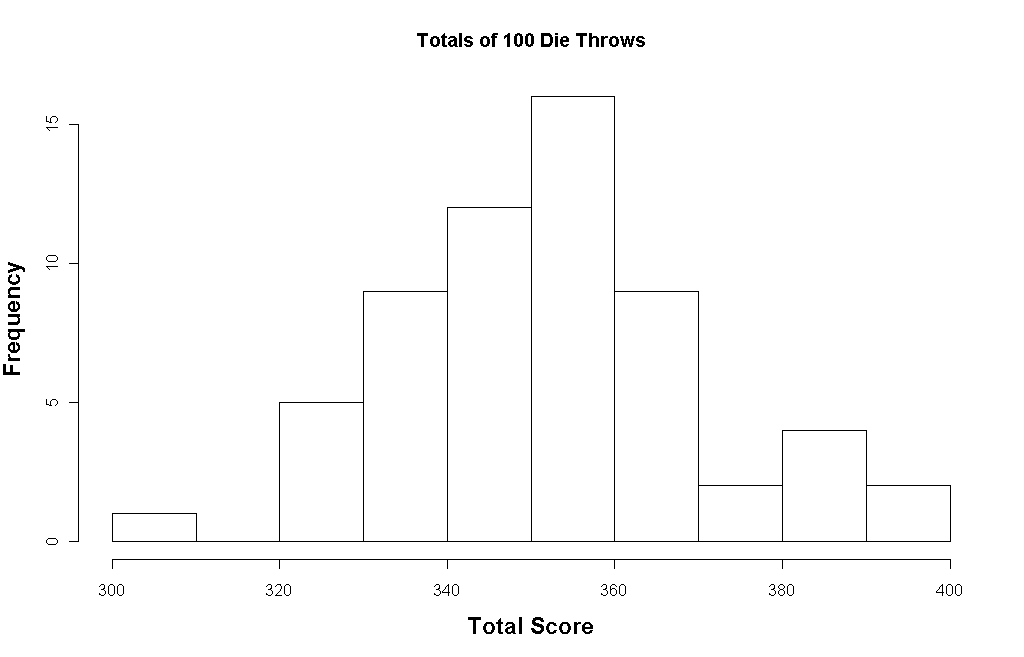
\includegraphics[scale=0.30]{images/3aDieHist}
%\end{center}
%

%--------------------------------------%
 \subsubsection{Constructing Histograms}
\begin{itemize}
\item Compute an appropriate number of class intervals.
\item As a rule of thumb, the number of class intervals is usually approximately the square root of the number of observations.
\item As there are 60 observations, we would normally use 7 or 8 class intervals.
\item To save time, we will just use 5 class intervals.
\end{itemize}



%---------------------------% \frametitle{Histograms}

%\begin{center}
%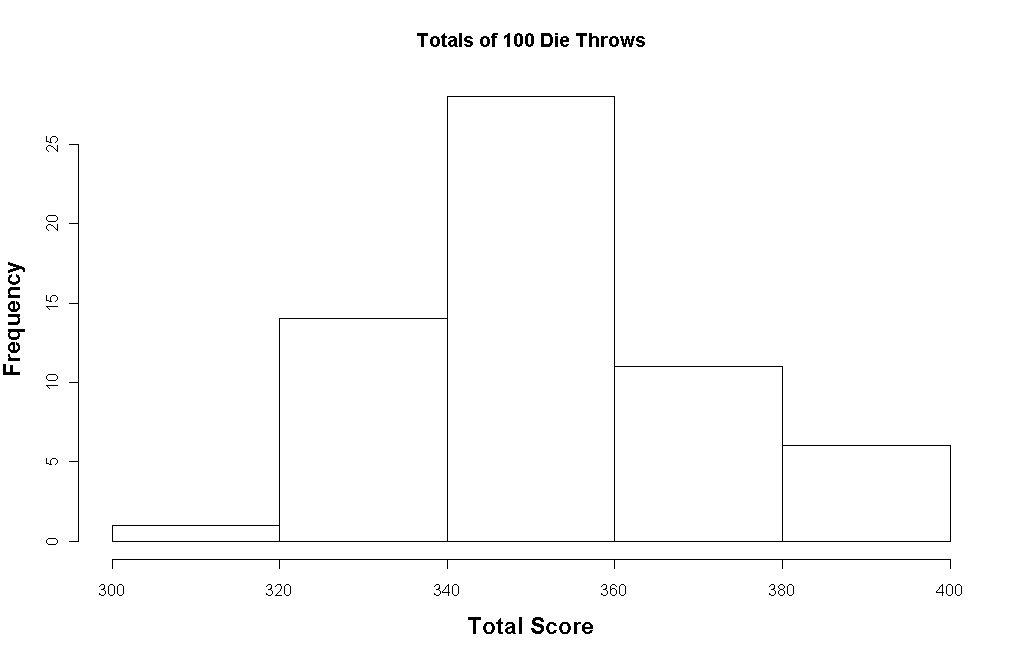
\includegraphics[scale=0.30]{images/3aDieHist2}
%\end{center}
%



\begin{itemize}
\item Suppose that the experiment of throwing a die 100 times and recording the total was repeated 100,000 times.
\item (If implemented on a computer, we would call this a simulation study)
\item The histogram of data (with a class interval width of 2) is shown on the next slide.
\item How should the shape of the histogram be described?
\item ``Bell-shaped" would be a suitable description.
\end{itemize}


%\begin{center}
%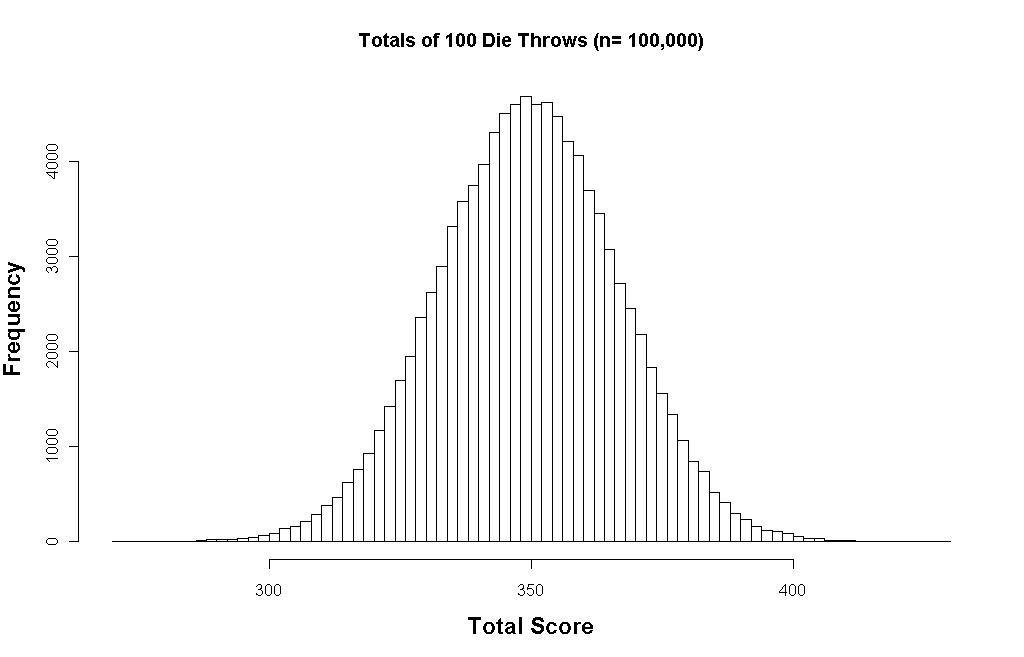
\includegraphics[scale=0.30]{images/3aDieHist3}
%\end{center}


%--------------------------------------%
%---------------------------% \frametitle{Simulation Study}
A couple of remarks about the simulation study, some of which will be relevant later on.
\begin{itemize}
% \item Approximately 76\% of the values are between 330 and 370.
\item Approximately 68.7\% of the values in the simulation study are between 332 and 367.
\item Approximately 95\% of the values are between 316 and 383.
\item $2.5\%$ of the values output are less than 316.
\item $2.5\%$ of the values study output are greater than 383.
\item 175 values are greater than or equal to 400, whereas 198 values are less than or equal to 300.
\item Results such as these are unusual, but they are not impossible.
\end{itemize}





Consider the following statistical experiment. You flip a coin 2 times and count the number of times the coin lands on heads. This is a binomial experiment because:
\begin{itemize}
\item The experiment consists of repeated trials. We flip a coin 2 times.
\item Each trial can result in just two possible outcomes - heads or tails.
\item The probability of success is constant - 0.5 on every trial.
\item The trials are independent; that is, getting heads on one trial does not affect whether we get heads on other trials.
\end{itemize}




%=================================================%
